\chapter{Shearlets}

We want to be able to express efficiently Epipolar Plane Images that will reduce the number of minimum views needed to recover the light field of a scene; this task can be achieved by understanding the EPIs as signals and using signal processing machinery developed in the last twenty years, in this chapter we will explain in detail state-of-the-art methods on signal sparse-representation.

\bigskip

One can think a signal as a function (or something that can be represented as) that contains information about the behavior or attributes of some phenomenon \cite{Roland}, by this definition it actually could be a lot of things; it also depends the area you are working on, this definition will work or not. For example, in signal processing, arbitrary binary data streams are not considered as signals. For the sake of simplicity in this thesis we will agree to define a signal as a function that could represent video, image or audio and it will be either analog (evaluated with continuous parameters) or digital (evaluated with discrete parameters). 

\bigskip

In signal processing and applied harmonic analysis one can generally represent the signals in a space-time domain, but one cannot get always meaningful information in this representation; plenty of different signal transforms have been proposed along time, this transforms are obtained generally by finding basis of certain functional spaces (e.g. $L^2(\mathbb{R}^2)$) and present different features like sparse representation of signals that permits an efficient processing and storing of them. The most known signal transform for its effectiveness and tradition is the Fourier Transform, proposed by the French Mathematician Joseph Fourier, on his paper "Théorie analytique de la chaleur" in 1822 where he showed that some functiones could be written as an infinite sum of sines and cosines. 

\bigskip

If $f\in L^2(\mathbb{R}^n)$ then its Fourier transform $\hat{f}$ will be 
$$
\hat{f}(\xi) := \int_{\mathbb{R}^n}f(x)e^{-i\langle x,\xi\rangle}dx
$$

one can think of the coordinates $\xi$ of the Fourier space, as one can see the Fourier transform $\hat{f}$ just gives information about the frequencies contained in $f$, but not at which time they occur; moreover, small changes in the neighborhood of some point $x\in\mathbb{R}^n$ could change significantly its Fourier transform, in general one would not like that. A small solution for this issue is reflected in the short-time Fourier transform; whose mechanism is based in localization of the Fourier transform to a certain window of $f$ and then move the window through the whole domain. Let $g\in L^2(\mathbb{R})$ the window function, the short-time Fourier transform of $f\in L^2(\mathbb{R})$ associated with the window $g$ will be

$$
S_gf(t,\xi)=\int_{\mathbb{R}} f(x)\overline{g(x-t)}e^{-ix\xi}dx=\langle f,M_{\xi}T_tg\rangle = (\widehat{f\cdot T_t\overline{g}})(\xi)\text{,  } t,\xi\in\mathbb{R}
$$

where $T_t:L^2(\mathbb{R})\longrightarrow L^2(\mathbb{R})$ is the translation operator with parameter $t$, given by 
$$
T_tf(x)=f(x-t)
$$
and $M_{\xi}:L^2(\mathbb{R})\longrightarrow L^2(\mathbb{R})$ is the modulation operator, given by 
$$
M_{\xi} f(x)=e^{i\xi x}f(x)
$$

\bigskip 

One can associate to this transform the atoms $\{M_{\xi}T_tg\}_{(t,\xi)\in\mathbb{R}^2}$; for computational purposes one can discretize the transform taking $(t,\xi)\in\Lambda=a\mathbb{Z}\times b\mathbb{Z}$ for some $a,b>0$; the resulting atoms $G(g,a,b):=\{g_{am,bn}=M_{bn}T_{am}\}_{(m,n)\in\mathbb{Z}}$, for some cases of $(a,b)\in\mathbb{R}$ $G(g,a,b)$ is a generating set of $L^2(\mathbb{R})$ with an explicit recovery formula with other features, such sequence of function are known as \textbf{frames} and can be understand as the generalization of orthonormal bases, we will study them in detail on the Section~\ref{sec:ShearletsFrames}, for a further reading about Gabor frames one can check \cite{Gabor}.

\bigskip

We introduced Gabor frames to overcome some limitations of the Fourier transform; Gabor frames also present some limitations
\begin{itemize}
\item When the Gabor frame is also a orthonormal bases don't have a good time-frequency localization \cite{Gabor}.
\item The size of the window $g$ does not change so Gabor frames are not sensible to very localized information, so for instance they will never detect a singularity or regularity information of a function.
\end{itemize} 
both limitations above can be overcome using \textbf{wavelets}.

\bigskip 

The concept of wavelets and the signal transform related was introduced first time 
in 1980s by the french mathematicians Morlet and Grossmann to refer to "small wave" (or \textit{ondelette} in french) when they were studying siesimic waves (check the original paper \cite{Grossman}). The \textit{continuous wavelet transform} of a function $f\in L^2(\mathbb{R})$ associated to a mother function $\psi\in L^2(\mathbb{R})$ is defined by 

$$
\begin{aligned}
\mathcal{W}_{\psi}f(a,b)&=\int_{\mathbb{R}}f(t)a^{-\frac{1}{2}}\overline{\psi\left(\frac{t-b}{a}\right)}dt\\
&=\langle f, T_bD_a\psi\rangle = (f\ast D_a\overline{\psi}^*)(b)\text{, } (a, b)\in\mathbb{R}^+\times\mathbb{R} 
\end{aligned}
$$

where $D_a:L^2(\mathbb{R}\longrightarrow L^2(\mathbb{R})$ is the dilation operator given by $D_a f(t)=a^{-\frac{1}{2}}f\left(\frac{t}{a}\right)$, and $f^*(t)=f(-t)$, $a$ is the scaling paramter (controls the size of the window) and $b$ is the translation parameter. If the mother function $\psi$ satisfy the admissibility condition 

$$
C_{\psi}:=\int_0^{\infty}\frac{|\hat{\psi}(\xi)|^2}{\xi}d\xi <\infty
$$

we will say that $\psi$ is a admissible wavelet. If one has an admissible wavelet, one can get an straightforward inversion or recovery formula as
$$
f=\frac{1}{C_{\psi}}\int_{\mathbb{R}}\int_0^{\infty} W_{\psi}f(a,b)T_bD_a\psi\frac{da}{a^2}db
$$

\bigskip

The sequence of wavelet atoms will be $\{\psi_{a,b}(t)=a^{-\frac{1}{2}}\overline{\psi\left(\frac{t-b}{a}\right)}\}_{(a,b)\in\mathbb{R}^+}$, so one can write the wavelet transform of $f$ as $W_{\psi}f(a,b)=\langle f,\psi_{a,b}\rangle$. One can discretize the wavelet transforms as by the inner product with the discrete set of wavelet atoms
$$
\psi_{j,m}(t):=a^{-\frac{1}{2}}\psi(a^{-j}t-bm)\text{,  } (j,m)\in\mathbb{Z}^2\text{,  } t\in \mathbb{R}\text{,   }(a,b)\in\mathbb{R}^+\times\mathbb{R}
$$

the set of discrete set of wavelet atoms is referred as wavelet system. Wavelets are very relevant in Signal Processing due their great features 
\begin{itemize}
\item One can get information about the regularity of a function $f$ by estimating bounds of its wavelet transform.
\item The scaling parameter permits us to detect very localized information, in particular is very effective detecting one dimensional singularities, this property leads to the construction of a Multiresolution Analysis (MRA) which is an important area in applied harmonic analysis(check \cite{Mallat} p. 264).
\item The unified treatment of both digital and continuous transforms permits an easy implementation.
\item It can represent sparsely one dimensional signals, in the sense that not a lot of coefficients will be significant so one can  them.
\end{itemize}

\bigskip

Over all the features that we just mentioned the one that gave most of its fame to the wavelet transform is the last one, i.e.\ sparse representation of one dimensional signals, for instance this porperty of wavelets is what the image compression standard JPEG 2000 is based on. It is worth it to study in more detail sparse representation of data.

\bigskip

It is not surprising that compression of data takes an important place in the academic research and industrial agenda nowadays. Our society generates and acquire a lot of data everyday that comes in a lot of different types and dimensions; the complexity of the processing of this raw data to extract some useful data in an understandable language grows with the dimensionality and size of the data. Even though, almost all data found in practical applications has the property that the relevant information which needs to be extracted or identified is sparse, that is, data are typically highly correlated and the essential information lives in lower dimensional subspaces (or manifolds). This information can be then captured using just few terms in an appropriate dictionary (e.g.\ some frame or orthonormal basis). 

\bigskip

The sparse representation property of data is important not only for data storage and transmission but also for feature extraction, classification, and other high-level tasks; finding a dictionary which sparsely represents a certain data class involves deep understanding of its dominant properties, which are typically associated with their geometric properties; for a deep treatment of this one can read \cite{IntroShearlets} and \cite{Gitta-Lim}.

\bigskip

So far we have just mentioned the sparse representation property for one-dimensional signals and also the existence of straight forward and fast algorithmic implementations; the latter is based in the general machinery to construct orthonormal wavelet bases known as \textit{Multiresolution Analysis} (MRA). In the one dimensional case, this is defined as a sequence of closed subspaces $(V_j)_{j\in\mathbb{Z}}$ in $L^2(\mathbb{R})$ known as the scaling spaces which satisfies the following properties

\begin{enumerate}
\item[(a)] $\{0\}\subset\ldots\subset V_{-2}\subset V_{-1}\subset V_0\subset V_1\subset V_2\subset\ldots L^2(\mathbb{R})$.
\item[(b)] $\cap_{j\in\mathbb{Z}}V_j=\{0\}$ and $\overline{\cup_{j\in\mathbb{Z}V_j}}=L^2(\mathbb{R})$.
\item[(c)] $f\in V_j$ if and only if $D_2^{-1}f\in V_{j+1}$.
\item[(d)] There exists a $\varphi\in L^2(\mathbb{R})$, called \textit{scaling function}, such that $\{T_m\varphi:m\in\mathbb{Z}\}$ is an orthonormal basis for $V_0$.
\end{enumerate}

This enables the decomposition of functions into different "resolution" levels associated with the so called wavelet spaces $W_j$, $j\in\mathbb{Z}$ which are defined by considering the orthogonal complements
$$
W_j:= V_{j+1}\ominus V_j\text{,  } j\in\mathbb{Z}
$$

This Multiresolution Analysis let us not only to decompose $L^2(\mathbb{R})$ as a direct sum of wavelet spaces but also gives us an alternative orthonormal basis with both the wavelet and the scaling fuction, of the form

$$
\{\varphi_m=T_m\varphi=\varphi(\cdot-m):m\in\mathbb{Z}\}\cup\{\psi_{j,m}:j\geq 0,m\in\mathbb{Z}\}
$$

where the scaling function take care of the low-frequency region $V_0$ and the wavelet terms of the complementary space $L^2(\mathbb{R})\ominus V_0$. One can read \cite{Mallat}. 

\bigskip

In this thesis we are interested in image processing, if one would like to apply wavelets to imaging science an extension of the theory to $L^2(\mathbb{R}^2)$. For a painless extension we can introduce the concept of tensor products of Hilbert spaces. If $\mathcal{H}_1$ and $\mathcal{H}_2$ are two Hilbert spaces the tensor product is a bilinear operator $\otimes:\mathcal{H}_1\times\mathcal{H}_2\longrightarrow \mathcal{H}_1\otimes\mathcal{H}_2$ where $\mathcal{H}_1\otimes\mathcal{H}_2$ is a new Hilbert space.

\bigskip

We can use strongly the fact that the tensor product of orthonormal bases is an orthonormal basis of $\mathcal{H}_1\otimes\mathcal{H}_2$. In the case of $\mathcal{H}_1=\mathcal{H}_2=L^2(\mathbb{R})$ and $f,g\in L^2(\mathcal{R})$,

$$
(f\otimes g)(x_1,x_2)=f(x_1)g(x_2)\text{,  } (x_1,x_2)\in\mathbb{R}^2,
$$

and $\mathcal{H}_1\otimes\mathcal{H}_2=L^2(\mathbb{R}^2)$. This concepts leads to the next theorem.

\bigskip

\begin{thm}[Two-dimensional wavelets]
Let $(V_j)_{j\in\mathbb{Z}}$ be an MRA for $L^2(\mathbb{R})$ with scaling function $\varphi\in L^2(\mathbb{R})$ and associated wavelet $\psi\in L^2(\mathbb{R})$. For $(x_1,x_2)\in\mathbb{R}^2$, we define
$$
\begin{aligned}
&\psi^1(x_1,x_2):=\varphi(x_1)\psi(x_2),\\
&\psi^2(x_1,x_2):=\psi(x_1)\varphi(x_2),\\
&\psi^3(x_1,x_2):=\psi(x_1)\psi_(x_2)
\end{aligned}
$$
Then 
$$
\{\psi_{j,m}^k(x_1,x_2)=2^{-j}\psi^k(2^{-j}x_1-m_1,2^{-j}x_2-m_2)\text{: } m=(m_1,m_2)\in\mathbb{Z}^2,k=1,2,3\}
$$
is an orthonormal basis for the wavelet space $W^2_j$, given by $V^2_j\oplus W^2_j=V^2_{j-1}$. Moreover,
$$
\{\psi_{j,m}^k\text{:  }j\in\mathbb{Z},m=(m_1,m_2)\in\mathbb{Z}^2,k=1,2,3\}
$$
is an orthonormal basis for $L^2(\mathbb{R}^2)$.
\end{thm}
\begin{proof}
One can find the proof on \cite{Mallat}, pp. 340-346.
\end{proof}

\bigskip

There exists more general non-separable two dimensional wavelets transforms using the continuous affine group to generalize the dilation operator $D_a$ to $D_M$ for two-dimensional invertible matrices $M$. The traditional theory of wavelets is based on the use of isotropic dilations and therefore is esentially a one-dimensional theory, so it is unable to give additional information about the geometry of the set of singularities of a function or distribution that are multivariate. The main problem is that the isotropic wavelet transform is simple but lacks of directional sensitivity and the ability to detect the multidimensional geometry of a function or distribution $f$.

\bigskip

One can formalize this notion using the concept of best $N$-term approximation. We will provide the general definition applied to dictionaries (collection of vectors on a Hilbert space $\{\varphi_i: i\in I\}\subset \mathcal{H}$ with $I$ finite or countable infinite).

\bigskip

\begin{defn}[Best N-term Approximation]
Let $D:=\{\varphi_i\text{:  }i\in I\}\subset \mathcal{H}$ be a dictionary. Consider a vector $x\in\mathcal{H}$ and an integer $N\in\mathbb{N}$. Then the \textit{best N-term approximation of x} with respect to $D$ is defined by the solution of the following minimization problem:
$$
\min_{I_N,(c_i)_{i\in I_N}}||x-\sum_{i\in I_N} c_i\varphi_i|| \text{ subject to } I:N\subset I,\# I_N\leq N
$$
\end{defn}

\bigskip

The best N-term approximation $f_N$ of $f\in L^2(\mathbb{R}^2)$ with respect to the dictionary formed by the wavelet basis can be understan as the obtained by approximating $f$ from its $N$ largest wavelet coefficients in magnitude. Let $\Lambda_N$ the index set corresponding to the $N$- largest wavelet coefficients $|\langle f,\psi_{\lambda}\rangle|$ associated with some wavelet basis $(\psi)_{\lambda\in\Lambda}$, the best $N$-term approximation will be
$$
f_N=\sum_{\lambda\in\Lambda_N}\langle f,\psi_{\lambda}\rangle\psi_{\lambda}
$$

\bigskip

To study the approximation of natural images by the wavelets, we first need to introduce a definition of what we will understand mathematically as a natural image, the so called \textit{cartoon-like functions}.

\bigskip

\begin{defn}[Cartoon-like functions]
The class of \textit{cartoon-like functions} $\mathcal{E}^2(\mathbb{R}^2)$ is defined as the set of functions $f:\mathbb{R}^2\longrightarrow \mathbb{C}$ of the form $f= f_0+\chi_B f_1$. Here, we assume that $B\subset [0,1]^2$ where $\partial B\in C^2$ and bounded curvature. Moreover, $f_i\in C^2(\mathbb{R}^2)$ with $||f_i||_{C^2}\leq 1$ and $\text{supp} f_i\subset [0,1]^2$ for $i=0,1$. 
\end{defn}

\bigskip

\begin{figure}[h!]
\centering
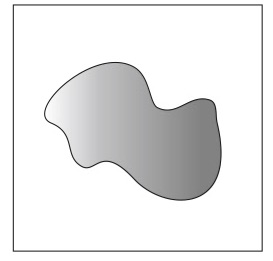
\includegraphics[width = 0.4 \textwidth]{./Diagrams/cartoon-like.jpg}
\caption{Example of a cartoon-like image. Figure taken from \cite{IntroShearlets} pp. 9}
\label{fig:cartoon-like}
\end{figure}

Now, let $f$ be a cartoon-like image containing a singularity along a smooth curve and $\{\psi_{j,m}\}$ be a standard wavelet bases of $L^2(\mathbb{R}^2)$. For $j$ sufficiently large, the only significan wavelet coefficients $\langle f,\psi_{ j,m}\rangle$ are the ones associated with the singularity. At each scale $2^{-j}$, each wavelet $\psi_{j,m}$ is supported inside a box of size $2^{-j}\times 2^{-j}$, there exist about $2^j$ elements of the wavelet basis overlapping the singularity curve. The associated wavelet coefficients are controlled by 

$$
|\langle f,	\psi_{j,m}\rangle|\leq ||f||_{\infty}||\psi_{j,n}||_{L^1(\mathbb{R}^2)}\lesssim 2^{-j}
$$

It follows that the $N$-th largest wavelet coefficient in magnitude, denoted by $\langle f,\psi_{j,m}\rangle_{(N)}$, is bounded by O($N^{-1}$). Thus, if $f$ is approximated by its best $N$-term approximation $f_N$, the $L^2$ error (called  best $N$-term approximation error) obeys

$$
\sigma_N(f,\{\psi_{j,m}\}_{j,m}^2=||f-f_N||^2_{L^2(\mathbb{R}^2)}\leq \sum_{\ell\geq N}|\langle f,\psi_{j,m}\rangle_{(l)}|^2\lesssim N^{-1}
$$

This estimate is actually tight, in the sense that there exist cartoon-like images for which the best $N$-term approximation error is

$$
\sigma_N(f,\{\psi_{j,m}\}_{j,m})\approx N^{-\frac{1}{2}}
$$
the proof of this result can be founded in \cite{Mallat}.

Even this looks like a nice result, it is far from optimal.

\bigskip

\begin{thm}
\label{C3S2T1}
Let $\{\psi_{\lambda}\}_{\lambda\in\Lambda}\subset L^2(\mathbb{R}^2)$ be a frame for $L^2(\mathbb{R}^2)$. Then the optimal best $N-term$ approximation error for any $f\in\mathcal{E}^2(\mathbb{R}^2)$ is
$$
\sigma_N(f,\{\psi_{\lambda}\}_{\lambda\in\Lambda})=O(N^{-1})
$$
\end{thm}
\begin{proof}
In Section~\ref{sec:ShearletsFrames} we will define the concept of frame. This result was proved by Donoho in 2001 on \cite{DonohobestNterm}, so one can refer to his proof.
\end{proof}

\bigskip

As we mentioned before, the problem with wavelets that does not make them to approach efficiently multivariate data is related to its isotropic scaling characteristic that makes them not sensible to directions. The question that can arise is, "Why should we care about anisotropic features related to multidimensional singularities?"; all the multivariate data are typically dominated by anisotropic features such as singularities on lower dimensional embedded manifolds; for example by edges in natural images or shock fronts in the solutions of transport equations. 

\begin{figure}[h!]
\centering
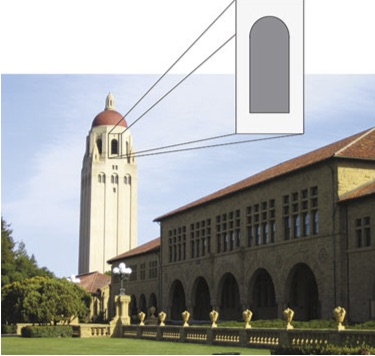
\includegraphics[width = 0.7\textwidth]{./Diagrams/edges-images.jpg}
\caption{Natural images governed by anisotropic structures. Figure taken from \cite{IntroShearlets} pp. 8}
\label{edges-images}
\end{figure}

\bigskip

The bound result of theorem~\ref{C3S2T1} works as a benchmark for optimally sparse approximation of two-dimensional data in form of cartoon-like functions. Moreover, to proof theorem~\ref{C3S2T1} Donoho used adapted triangulations, which suggests that analyzing elemnts with elongated and orientable supports are required to get optimally sparse approximations of piecewise smooth two-dimensional functions. This observation leaded to two different approaches for solving this problem, the curvelets (proposed by E. Candès and D. Donoho in 1999 \cite{Curvelets}), and the shearlets (proposed by Kanghui Guro, Gitta Kutyniok and Demetrio Labate in 2005 \cite{FirstShearlets}), both are able to achieve the same optimal approximation rate; the one used in this thesis to sparsely represent EPIs is the latter due the possibility to develope a faithful implementation. 

\section{Shearlet Systems and Transform}

We just discussed the limitations of wavelet systems in higher dimensions, we will then the concept of shearlet systems as a framework to solve these limitations. We also mentioned that in order to achieve optimally sparse approximations of signals with anisotropic singularities such as cartoon-like images, the analyzing elements must be made by waveforms ranging over several scales, orientations, and locations with the ability to become very elongated. One need then the combination of an appropriate scaling operator to generate elements at different scales, an orthogonal operator to change their orientations, and a translation operator to displace the elements over the two-dimensional plane. 

\bigskip

By tradition and effectivenes one can use the family of dilation operators $D_{A_a}$, $a>0$ based on parabolic scaling matrices $A_a$ of the form

$$
A_a:=
\left(
\begin{matrix}
a & 0 \\
0 & a^{1/2}
\end{matrix}
\right)
$$

This is the first approach to a scaling operator by the long history of parabolic scaling in harmonic analysis literature \cite{Fefferman}; the so called \textit{Classical Shearlets} use this approach, one can generalize the scaling using matrices of the form 

$$
A_a:=
\left(
\begin{matrix}
a & 0 \\
0 & a^{\alpha}
\end{matrix}
\right)
$$

with $\alpha\in (0,1)$ that controls the "degree of anisotropy" and the generated system is known as \textit{Alpha Particle}, we will discuss this in detail on Section~\ref{sec:AlphaShearlets}. Parabolic scaling is also knwon to be required in order to obtain optimally sparse approximations of cartoon-like images, since it is the best adapted to $C^2$-regularity of the curves of discontinuity, i.e.\ is efficient to approximate smooth curves, moreover choosing $a=2$ gives the best performance.

\bigskip

 Next, we need an orthogonal transformation to change to change the orientation of the waveforms. One does not use rotations since it destroys the structure of the integer lattice $\mathbb{Z}^2$ whenever the rotation angle is different from $0,\pm\frac{\pi}{2},\pm\frac{3\pi}{2}$, which will represent an issue in the discrete setting. One chooses the shearing operator $D_s$, $s\in\mathbb{R}$, where the \textit{shearing matrix} $S_s$ is given by 
$$
S_s=
\left(
\begin{matrix}
1 & s \\
0 & 1
\end{matrix}
\right)
$$

\begin{figure}[h!]
\centering
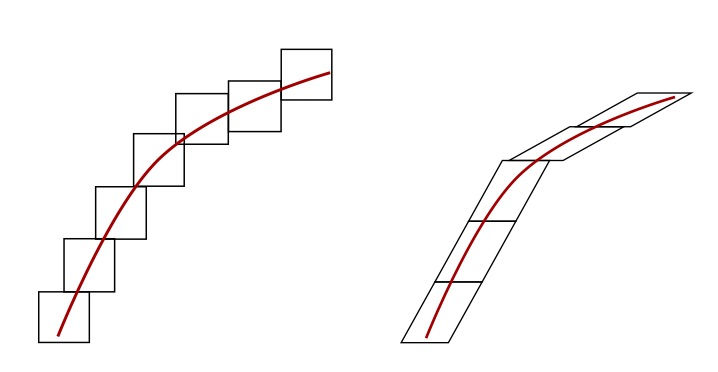
\includegraphics[width = 0.7\textwidth]{./Diagrams/anisotropic_isotropic.jpg}
\caption{Optimal covering og anisotropic scaled and sheared atoms}
\label{edges-images}
\end{figure}

\section{Shearlets as Frames}
\label{sec:ShearletsFrames}

\section{Generalization of Shearlets to Alpha Particles}
\label{sec:AlphaShearlets}

\section{Linear Shearlets and its relation with ridgelets}

\section{Image inpainting using Shearlets}

\section{Epipolar-plane representation with linear Shearlets}
